\chapter{Исследовательская часть}

В данном разделе будут приведены примеры работы программы, а также проведен сравнительный анализ алгоритмов при различных ситуациях на основе полученных данных.

\section{Технические характеристики}

Технические характеристики устройства, на котором выполнялось тестирование представлены далее:
\begin{itemize}[label={---}]
	\item операционная система: Windows 11, x64;
	\item оперативная память: 8 Гб;
	\item процессор: AMD Ryzen 5 5500U с видеокартой Radeon Graphics 2.10~ГГц.
\end{itemize}

Во время замеров времени ноутбук был нагружен только встроенными приложениями окружения.

\section{Демонстрация работы программы}

На рисунке~\ref{img:run} представлен результат работы программы.

\begin{figure}[H]
	\center{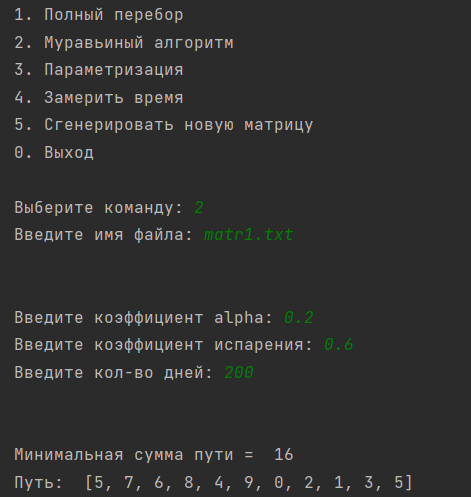
\includegraphics[scale=1.5]{img/run}}
	\caption{Пример работы программы}
	\label{img:run}
\end{figure}
\clearpage

\section{Время выполнения алгоритмов}

Как было сказано выше, используется функция замера процессорного времени \textit{process\_time} из библиотеки \textit{time} на \textit{Python}. Функция возвращает пользовательское процессорное время типа \textit{float}.

Использовать функцию приходится дважды, затем из конечного времени нужно вычесть начальное, чтобы получить результат.

Замеры проводились для размеров матрицы от 2 до 10 с шагом 1 по 10 раз на различных входных данных.

Результаты замеров приведены в таблице~\ref{tbl:time_mes} (время в с).

\begin{table}[H]
	\begin{center}
		\begin{threeparttable}
			\captionsetup{justification=raggedright, singlelinecheck=off}
			\caption{Результаты замеров времени}
			\label{tbl:time_mes}
			\begin{tabular}{|c|r|r|}
				\hline
				Размер матрицы & Полный перебор, с&Муравьиный алгоритм, с\\ \hline
				2 &   0.000019 &   0.004641 \\ \hline
				3 &   0.000053 &   0.013441 \\ \hline
				4 &   0.000075 &   0.032406 \\ \hline
				5 &   0.000313 &   0.065612 \\ \hline
				6 &   0.001941 &   0.132931 \\ \hline
				7 &   0.025000 &   0.226562 \\ \hline
				8 &   0.153125 &   0.371875 \\ \hline
				9 &   1.481250 &   0.556250 \\ \hline
				10 &  16.020312 &   0.801562 \\ \hline
			\end{tabular}
		\end{threeparttable}
	\end{center}
\end{table}


На рисунке~\ref{img:graph} приведена визуализация результатов замеров.

\inputPdf{graph}{Визуализация результатов замеров}

\section{Параметризация}

Параметризация была проведена на классе данных, состоящем из трех матриц размером $10\times10$. Муравьиный алгоритм был запущен для всех значений $\alpha, \rho \in [0; 1]$ с шагом 0.2.
В качестве эталонного значения был взят результат работы алгоритма
полного перебора.

Далее будут представлены матрицы, на которых происходила параметризация и таблицы с результатами её выполнения.

В качестве класса данных были взяты матрицы, в которых все значения незначительно отличаются друг от друга и находятся в
диапазоне [1, 8].

\begin{equation}
	\label{eq:kd1}
	M_{1} = \begin{pmatrix}
		0 & 1 & 3 & 1 & 1 & 2 & 7 & 6 & 4 & 5 \\ 
		8 & 0 & 8 & 7 & 3 & 7 & 6 & 2 & 7 & 7 \\
		5 & 1 & 0 & 5 & 4 & 4 & 4 & 8 & 4 & 3 \\
		8 & 7 & 7 & 0 & 3 & 6 & 1 & 2 & 8 & 2 \\
		6 & 2 & 2 & 7 & 0 & 8 & 1 & 7 & 3 & 2 \\
		5 & 8 & 8 & 7 & 2 & 0 & 2 & 5 & 2 & 7 \\
		7 & 2 & 4 & 8 & 7 & 4 & 0 & 8 & 6 & 5 \\
		5 & 7 & 2 & 2 & 7 & 4 & 1 & 0 & 6 & 5 \\
		7 & 6 & 3 & 3 & 1 & 7 & 2 & 2 & 0 & 8 \\
		4 & 2 & 6 & 6 & 1 & 8 & 4 & 3 & 8 & 0 
	\end{pmatrix}
\end{equation}

\begin{equation}
	\label{eq:kd1}
	M_{2} = \begin{pmatrix}
		0 & 7& 4& 7& 1& 3& 1& 1& 2& 3 \\
		6& 0& 5& 5& 3& 2& 6& 8& 3& 3 \\
		7& 6& 0& 2& 1& 1& 5& 7& 1& 8 \\
		7& 7& 5& 0& 1& 3& 8& 8& 6& 8 \\
		8& 4& 7& 5& 0& 4& 8& 1& 4& 5 \\
		7& 7& 7& 3& 8& 0& 3& 3& 4& 3 \\
		6& 6& 6& 2& 4& 3& 0& 4& 4& 3 \\
		4& 2& 3& 6& 2& 4& 3& 0& 8& 2 \\
		1& 5& 4& 8& 8& 8& 4& 3& 0& 4 \\
		4& 1& 4& 3& 2& 3& 3& 7& 5& 0 
	\end{pmatrix}
\end{equation}

\begin{equation}
	\label{eq:kd1}
	M_{1} = \begin{pmatrix}
		0& 2& 7& 3& 5& 8& 2& 3& 4& 1 \\
		4& 0& 4& 2& 3& 4& 7& 2& 7& 2 \\
		7& 2& 0& 6& 6& 3& 2& 3& 4& 8 \\
		7& 6& 1& 0& 4& 3& 7& 3& 6& 2 \\
		5& 1& 8& 4& 0& 5& 1& 8& 5& 3 \\
		3& 7& 3& 6& 1& 0& 5& 1& 2& 7 \\
		2& 1& 5& 8& 5& 5& 0& 1& 3& 1 \\
		6& 3& 7& 7& 8& 5& 8& 0& 7& 5 \\
		6& 1& 3& 3& 4& 6& 5& 4& 0& 7 \\
		6& 5& 4& 6& 3& 2& 2& 7& 5& 0 
		
	\end{pmatrix}
\end{equation}

В таблице \ref{tbl:par} представлены результаты параметризации.
\begin{longtable}{|c|c|c|c|c|c|c|}
	\captionsetup{justification=raggedright,singlelinecheck=false}
	\caption{\label{tbl:par}Результаты параметризации}\\
	
	\hline
	$\alpha$ & $\rho$ & Количество дней & Результат 1 & Результат 2 & Результат 3 & $\max$\\
	\hline
	0.0 &  0.0 &    1 &    12 &    12 &     8 &    12 \\
	0.0 &  0.0 &   10 &     5 &     5 &     3 &     5 \\
	0.0 &  0.0 &   50 &     1 &     0 &     1 &     1 \\
	0.0 &  0.0 &  100 &     0 &     0 &     2 &     2 \\
	0.0 &  0.0 &  500 &     0 &     0 &     0 &     0 \\ \hline
	0.0 &  0.2 &    1 &    13 &    16 &    10 &    16 \\
	0.0 &  0.2 &   10 &     2 &     4 &     2 &     4 \\
	0.0 &  0.2 &   50 &     1 &     1 &     2 &     2 \\
	0.0 &  0.2 &  100 &     0 &     2 &     0 &     2 \\
	0.0 &  0.2 &  500 &     0 &     0 &     0 &     0 \\ \hline
	0.0 &  0.4 &    1 &    12 &    10 &     9 &    12 \\
	0.0 &  0.4 &   10 &     4 &     7 &     3 &     7 \\
	0.0 &  0.4 &   50 &     0 &     0 &     2 &     2 \\
	0.0 &  0.4 &  100 &     1 &     0 &     2 &     2 \\
	0.0 &  0.4 &  500 &     0 &     0 &     0 &     0 \\ \hline
	0.0 &  0.6 &    1 &     3 &     8 &     2 &     8 \\
	0.0 &  0.6 &   10 &     3 &     3 &     4 &     4 \\
	0.0 &  0.6 &   50 &     0 &     0 &     1 &     1 \\
	0.0 &  0.6 &  100 &     1 &     0 &     1 &     1 \\
	0.0 &  0.6 &  500 &     0 &     0 &     0 &     0 \\ \hline
	0.0 &  0.8 &    1 &    10 &    10 &    11 &    11 \\
	0.0 &  0.8 &   10 &     2 &     0 &     3 &     3 \\
	0.0 &  0.8 &   50 &     1 &     0 &     2 &     2 \\
	0.0 &  0.8 &  100 &     1 &     0 &     0 &     1 \\
	0.0 &  0.8 &  500 &     0 &     0 &     0 &     0 \\ \hline
	0.0 &  1.0 &    1 &    10 &     8 &     2 &    10 \\
	0.0 &  1.0 &   10 &     1 &     4 &     4 &     4 \\
	0.0 &  1.0 &   50 &     2 &     2 &     2 &     2 \\
	0.0 &  1.0 &  100 &     1 &     2 &     0 &     2 \\
	0.0 &  1.0 &  500 &     0 &     0 &     0 &     0 \\ \hline
	0.2 &  0.0 &    1 &    12 &    13 &    15 &    15 \\
	\hline
	\pagebreak
	\multicolumn{7}{l}{\textit{Продолжение таблицы}}\\
	\hline
	0.2 &  0.0 &   10 &     7 &    10 &     5 &    10 \\
	0.2 &  0.0 &   50 &     4 &     1 &     2 &     4 \\
	0.2 &  0.0 &  100 &     1 &     0 &     1 &     1 \\
	0.2 &  0.0 &  500 &     1 &     0 &     0 &     1 \\ \hline
	0.2 &  0.2 &    1 &    10 &    10 &    11 &    11 \\
	0.2 &  0.2 &   10 &     5 &     7 &     3 &     7 \\
	0.2 &  0.2 &   50 &     1 &     2 &     2 &     2 \\
	0.2 &  0.2 &  100 &     0 &     1 &     1 &     1 \\
	0.2 &  0.2 &  500 &     0 &     0 &     1 &     1 \\ \hline
	0.2 &  0.4 &    1 &    14 &     9 &    10 &    14 \\
	0.2 &  0.4 &   10 &     4 &     5 &     3 &     5 \\
	0.2 &  0.4 &   50 &     1 &     2 &     2 &     2 \\
	0.2 &  0.4 &  100 &     1 &     0 &     1 &     1 \\
	0.2 &  0.4 &  500 &     0 &     0 &     0 &     0 \\ \hline
	0.2 &  0.6 &    1 &    10 &     7 &     5 &    10 \\
	0.2 &  0.6 &   10 &     4 &     3 &     5 &     5 \\
	0.2 &  0.6 &   50 &     3 &     0 &     2 &     3 \\
	0.2 &  0.6 &  100 &     0 &     2 &     1 &     2 \\
	0.2 &  0.6 &  500 &     0 &     0 &     0 &     0 \\ \hline
	0.2 &  0.8 &    1 &    10 &    17 &     6 &    17 \\
	0.2 &  0.8 &   10 &     7 &     1 &     4 &     7 \\
	0.2 &  0.8 &   50 &     1 &     4 &     2 &     4 \\
	0.2 &  0.8 &  100 &     1 &     0 &     2 &     2 \\
	0.2 &  0.8 &  500 &     1 &     0 &     0 &     1 \\ \hline
	0.2 &  1.0 &    1 &     9 &    18 &     8 &    18 \\
	0.2 &  1.0 &   10 &     5 &     4 &     3 &     5 \\
	0.2 &  1.0 &   50 &     2 &     3 &     4 &     4 \\
	0.2 &  1.0 &  100 &     1 &     3 &     2 &     3 \\
	0.2 &  1.0 &  500 &     0 &     0 &     1 &     1 \\ \hline
	0.4 &  0.0 &    1 &     8 &    13 &     9 &    13 \\
	0.4 &  0.0 &   10 &     1 &     6 &     5 &     6 \\
	0.4 &  0.0 &   50 &     2 &     6 &     2 &     6 \\
	\hline
	\pagebreak
	\multicolumn{7}{l}{\textit{Продолжение таблицы}}\\
	\hline
	0.4 &  0.0 &  100 &     0 &     5 &     0 &     5 \\
	0.4 &  0.0 &  500 &     1 &     1 &     1 &     1 \\ \hline
	0.4 &  0.2 &    1 &    11 &    21 &     6 &    21 \\
	0.4 &  0.2 &   10 &     3 &     9 &     5 &     9 \\
	0.4 &  0.2 &   50 &     2 &     2 &     1 &     2 \\
	0.4 &  0.2 &  100 &     4 &     2 &     1 &     4 \\
	0.4 &  0.2 &  500 &     1 &     0 &     0 &     1 \\ \hline
	0.4 &  0.4 &    1 &    13 &    14 &     5 &    14 \\
	0.4 &  0.4 &   10 &     8 &     3 &     5 &     8 \\
	0.4 &  0.4 &   50 &     1 &     4 &     1 &     4 \\
	0.4 &  0.4 &  100 &     3 &     2 &     2 &     3 \\
	0.4 &  0.4 &  500 &     1 &     0 &     1 &     1 \\ \hline
	0.4 &  0.6 &    1 &    18 &     5 &     9 &    18 \\
	0.4 &  0.6 &   10 &     1 &     2 &     7 &     7 \\
	0.4 &  0.6 &   50 &     2 &     0 &     3 &     3 \\
	0.4 &  0.6 &  100 &     0 &     2 &     2 &     2 \\
	0.4 &  0.6 &  500 &     1 &     0 &     0 &     1 \\ \hline
	0.4 &  0.8 &    1 &    14 &    10 &     9 &    14 \\
	0.4 &  0.8 &   10 &     1 &     4 &     4 &     4 \\
	0.4 &  0.8 &   50 &     5 &     1 &     1 &     5 \\
	0.4 &  0.8 &  100 &     1 &     3 &     3 &     3 \\
	0.4 &  0.8 &  500 &     1 &     2 &     0 &     2 \\ \hline
	0.4 &  1.0 &    1 &    10 &    19 &     9 &    19 \\
	0.4 &  1.0 &   10 &     1 &     8 &     5 &     8 \\
	0.4 &  1.0 &   50 &     5 &     4 &     2 &     5 \\
	0.4 &  1.0 &  100 &     3 &     0 &     2 &     3 \\
	0.4 &  1.0 &  500 &     0 &     3 &     2 &     3 \\ \hline
	0.6 &  0.0 &    1 &    11 &    12 &     9 &    12 \\
	0.6 &  0.0 &   10 &     1 &    10 &     4 &    10 \\
	0.6 &  0.0 &   50 &     2 &     7 &     5 &     7 \\
	0.6 &  0.0 &  100 &     3 &     5 &     1 &     5 \\
	0.6 &  0.0 &  500 &     1 &     2 &     1 &     2 \\
	\hline
	\pagebreak
	\multicolumn{7}{l}{\textit{Продолжение таблицы}}\\
	\hline
	0.6 &  0.2 &    1 &     8 &    10 &    15 &    15 \\
	0.6 &  0.2 &   10 &     6 &    15 &     7 &    15 \\
	0.6 &  0.2 &   50 &     6 &     7 &     3 &     7 \\
	0.6 &  0.2 &  100 &     1 &     0 &     2 &     2 \\
	0.6 &  0.2 &  500 &     1 &     1 &     1 &     1 \\ \hline
	0.6 &  0.4 &    1 &     9 &    15 &     7 &    15 \\
	0.6 &  0.4 &   10 &     6 &     5 &     5 &     6 \\
	0.6 &  0.4 &   50 &     3 &     3 &     4 &     4 \\
	0.6 &  0.4 &  100 &     3 &     5 &     2 &     5 \\
	0.6 &  0.4 &  500 &     1 &     0 &     1 &     1 \\ \hline
	0.6 &  0.6 &    1 &     6 &    11 &     7 &    11 \\
	0.6 &  0.6 &   10 &     6 &     9 &     3 &     9 \\
	0.6 &  0.6 &   50 &     5 &     5 &     4 &     5 \\
	0.6 &  0.6 &  100 &     2 &     4 &     3 &     4 \\
	0.6 &  0.6 &  500 &     1 &     3 &     2 &     3 \\ \hline
	0.6 &  0.8 &    1 &    11 &    14 &     9 &    14 \\
	0.6 &  0.8 &   10 &     9 &    11 &     5 &    11 \\
	0.6 &  0.8 &   50 &     5 &     7 &     4 &     7 \\
	0.6 &  0.8 &  100 &     2 &     5 &     3 &     5 \\
	0.6 &  0.8 &  500 &     1 &     2 &     0 &     2 \\ \hline
	0.6 &  1.0 &    1 &    13 &    10 &     3 &    13 \\
	0.6 &  1.0 &   10 &     4 &    10 &     5 &    10 \\
	0.6 &  1.0 &   50 &     1 &     0 &     2 &     2 \\
	0.6 &  1.0 &  100 &     2 &     0 &     1 &     2 \\
	0.6 &  1.0 &  500 &     1 &     4 &     1 &     4 \\ \hline
	0.8 &  0.0 &    1 &    13 &    20 &    10 &    20 \\
	0.8 &  0.0 &   10 &     7 &    12 &     5 &    12 \\
	0.8 &  0.0 &   50 &     2 &     6 &     1 &     6 \\
	0.8 &  0.0 &  100 &     3 &     8 &     2 &     8 \\
	0.8 &  0.0 &  500 &     2 &     3 &     1 &     3 \\ \hline
	0.8 &  0.2 &    1 &    16 &    16 &    18 &    18 \\ 
	0.8 &  0.2 &   10 &    15 &     4 &     7 &    15 \\
	\hline
	\pagebreak
	\multicolumn{7}{l}{\textit{Продолжение таблицы}}\\
	\hline
	0.8 &  0.2 &   50 &     4 &     9 &     2 &     9 \\
	0.8 &  0.2 &  100 &     2 &     4 &     4 &     4 \\
	0.8 &  0.2 &  500 &     0 &     4 &     1 &     4 \\ \hline
	0.8 &  0.4 &    1 &    11 &    11 &     5 &    11 \\
	0.8 &  0.4 &   10 &     8 &    11 &     9 &    11 \\
	0.8 &  0.4 &   50 &     5 &     6 &     4 &     6 \\
	0.8 &  0.4 &  100 &     5 &     6 &     3 &     6 \\
	0.8 &  0.4 &  500 &     1 &     3 &     2 &     3 \\ \hline
	0.8 &  0.6 &    1 &    18 &     5 &    12 &    18 \\
	0.8 &  0.6 &   10 &     8 &    11 &     8 &    11 \\
	0.8 &  0.6 &   50 &     6 &     6 &     6 &     6 \\
	0.8 &  0.6 &  100 &     2 &     4 &     3 &     4 \\
	0.8 &  0.6 &  500 &     2 &     5 &     1 &     5 \\ \hline
	0.8 &  0.8 &    1 &    16 &    17 &    11 &    17 \\
	0.8 &  0.8 &   10 &     3 &    13 &     8 &    13 \\
	0.8 &  0.8 &   50 &     4 &     5 &     2 &     5 \\
	0.8 &  0.8 &  100 &     2 &     6 &     4 &     6 \\
	0.8 &  0.8 &  500 &     1 &     5 &     2 &     5 \\ \hline
	0.8 &  1.0 &    1 &    15 &    15 &    12 &    15 \\
	0.8 &  1.0 &   10 &     8 &    10 &     6 &    10 \\
	0.8 &  1.0 &   50 &     6 &     9 &     4 &     9 \\
	0.8 &  1.0 &  100 &     3 &     6 &     2 &     6 \\
	0.8 &  1.0 &  500 &     4 &     2 &     1 &     4 \\ \hline
	1.0 &  0.0 &    1 &     8 &    23 &     9 &    23 \\
	1.0 &  0.0 &   10 &     8 &     9 &     7 &     9 \\
	1.0 &  0.0 &   50 &     9 &     7 &     6 &     9 \\
	1.0 &  0.0 &  100 &     5 &     8 &     5 &     8 \\
	1.0 &  0.0 &  500 &     4 &     4 &     0 &     4 \\ \hline
	1.0 &  0.2 &    1 &     5 &    16 &    10 &    16 \\
	1.0 &  0.2 &   10 &     9 &     9 &     5 &     9 \\
	1.0 &  0.2 &   50 &     7 &     4 &     3 &     7 \\
	1.0 &  0.2 &  100 &     4 &     8 &     5 &     8 \\
	\hline
	\pagebreak
	\multicolumn{7}{l}{\textit{Продолжение таблицы}}\\
	\hline
	1.0 &  0.2 &  500 &     5 &     6 &     3 &     6 \\ \hline
	1.0 &  0.4 &    1 &    10 &    21 &    13 &    21 \\
	1.0 &  0.4 &   10 &     8 &    12 &     4 &    12 \\
	1.0 &  0.4 &   50 &     7 &     7 &     4 &     7 \\
	1.0 &  0.4 &  100 &     7 &     4 &     3 &     7 \\
	1.0 &  0.4 &  500 &     3 &     6 &     4 &     6 \\ \hline
	1.0 &  0.6 &    1 &    18 &    20 &    11 &    20 \\
	1.0 &  0.6 &   10 &     8 &    12 &     7 &    12 \\
	1.0 &  0.6 &   50 &     6 &     1 &     5 &     6 \\
	1.0 &  0.6 &  100 &     4 &     6 &     5 &     6 \\
	1.0 &  0.6 &  500 &     3 &     6 &     3 &     6 \\ \hline
	1.0 &  0.8 &    1 &    16 &    18 &    16 &    18 \\
	1.0 &  0.8 &   10 &    13 &    10 &     4 &    13 \\
	1.0 &  0.8 &   50 &     7 &     7 &     5 &     7 \\
	1.0 &  0.8 &  100 &     5 &     4 &     5 &     5 \\
	1.0 &  0.8 &  500 &     5 &     4 &     2 &     5 \\ \hline
	1.0 &  1.0 &    1 &    12 &    17 &    12 &    17 \\
	1.0 &  1.0 &   10 &     8 &    10 &     5 &    10 \\
	1.0 &  1.0 &   50 &     8 &     7 &     3 &     8 \\
	1.0 &  1.0 &  100 &     4 &     4 &     2 &     4 \\
	1.0 &  1.0 &  500 &     3 &     3 &     2 &     3 \\ \hline
	
\end{longtable}


\section{Вывод}

Как видно из графика \ref{img:graph}, реализация алгоритма полного перебора работает быстрее реализации муравьиного алгоритма при размерах матрицы меньше~9.

В связи с результатами параметризации можно сделать вывод, что оптимальными значениями параметров являются $\alpha = 0.2, \rho = 0.4, количество дней = 500$.